\chapter{Specifikacija programske potpore}
		
	\section{Funkcionalni zahtjevi}
			
			\noindent \textbf{Dionici:}
			
			\begin{packed_enum}
				
				\item Registrirani korisnik
				\begin{packed_enum}
				
				    \item Korisnik 
				    \item Vlasnik obrta
				    
				\end{packed_enum}
				\item Neregistrirani korisnik
				\item Razvojni tim
				
			\end{packed_enum}
			
			\noindent \textbf{Aktori i njihovi funkcionalni zahtjevi:}
			
			
			\begin{packed_enum}
				\item  \underbar{Neregistrirani/neprijavljeni korisnik  (inicijator) može:}
				
				\begin{packed_enum}
					
					\item na karti pregledati lokacije prikladne za pse 
					\item odabrati marker i dobiti prikaz općih informacija za lokaciju (ime lokacije, ocjena, vrsta) ili obrt (ime obrta, adresa, OIB, kontakt-broj, kratki opis, djelatnost)
                    \item vidjeti plaćene lokacije koje su dodatno istaknute
					\item unijeti specifičnu lokaciju na karti koja ga zatim centrira
					\item odabrati kategoriju čiji se markeri onda prikazuju
					\item stvoriti korisnički račun "Korisnik" za koji su mu potrebni korisničko ime, lozinka, e-mail
                    \item stvoriti korisnički račun "Vlasnik obrta" za koji su mu potrebni korisničko ime, lozinka, e-mail te podaci o obrtu i kartici
					
				\end{packed_enum}
			
				\item  \underbar{Običan korisnik (inicijator) može:}
				
				\begin{packed_enum}
					
					\item potvrditi e-mail o uspješnoj registraciji
					\item pregledavati i mijenjati osobne podatke
					\item izbrisati svoj korisnički račun 
					\item podijeliti svoje mišljenje o povoljnosti lokacije za pse
					\item unosom imena lokacije i odabirom njezine kategorije iz izbornika označiti lokaciju za koju želi iskazati mišljenje
					\item stvoriti lokaciju koju će označiti prikladnom ili neprikladnom
					
				\end{packed_enum}
				
				\item  \underbar{Vlasnik obrta (inicijator) može:}
				
				\begin{packed_enum}
					\item potvrditi e-mail o uspješnoj registraciji
                    \item pregledavati i mijenjati osobne podatke
					\item pregledavati i mijenjati podatke o svom obrtu
                    \item izbrisati svoj korisnički račun
					\item promovirati svoj obrt uz novčanu naknadu
					\item odgovoriti na recenzije korisnika
					
				\end{packed_enum}
				
				\item  \underbar{Baza podataka (sudionik):}
				
				\begin{packed_enum}
					
					\item pohranjuje sve podatke o korisnicima i njihovim ovlastima
					\item pohranjuje sve podatke o obrtima
					\item pohranjuje sve podatke o karticama
					
				\end{packed_enum}
				
				\item  \underbar{Karta (sudionik) može:}
				
				\begin{packed_enum}
				  
				  \item slati upit korisniku o njegovoj trenutnoj adresi
				  \item dohvatiti podatke iz baze podataka
				  \item prikazivati obrte i lokacije markerima
                  \item prikazivati informacije o lokacijama
				  
				\end{packed_enum}
				
			\end{packed_enum}
			
			\eject 	
			
				
			\subsection{Obrasci uporabe}
				
				\subsubsection{Opis obrazaca uporabe}
				
				\noindent \underbar{\textbf{UC1 - Registracija}}
					\begin{packed_item}
	
						\item \textbf{Glavni sudionik: } Neregistrirani korisnik
						\item  \textbf{Cilj:} Stvoriti korisnički račun za pristup sustavu 
						\item  \textbf{Sudionici:} Baza podataka
						\item  \textbf{Preduvjet:} -
						\item  \textbf{Opis osnovnog tijeka:}
						
						\item[] \begin{packed_enum}
	
							\item Neregistrirani korisnik u zaglavlju odabire opciju "Prijava"
							\item Odabire opciju "Registrirajte se"
							\item Odabire jednu od dvije mogućnosti registracije kao: korisnik ili vlasnik obrta
							\item Unosi tražene podatke (korisničko ime, e-mail, lozinka)
							\item[] \begin{packed_enum}
                                \item Ako je odabrao opciju vlasnik obrta unosi dodatne podatke o obrtu i kartici
							\end{packed_enum}
							\item Prima obavijest o uspješnoj registraciji putem e-maila
                            \item[] \begin{packed_enum}
                                \item Ako je odabrao opciju vlasnik obrta prima i e-mail s potvrdom o uspješnom plaćanju
							\end{packed_enum}
						\end{packed_enum}
						
						\item  \textbf{Opis mogućih odstupanja:}
						
						\item[] \begin{packed_item}
	
							\item[2.a] Odabir već zauzetog korisničkog imena/e-maila, unos podataka u nedozvoljenom formatu
							
							\item[] \begin{packed_enum}
								
								\item Sustav upozorava korisnika o neuspješnom unosu te ga vraća na stranicu za registraciju
								\item Korisnik mijenja potrebne podatke, završava unos ili odustaje od registracije
								
							\end{packed_enum}
							
						\end{packed_item}
					\end{packed_item}
					
				\noindent \underbar{\textbf{UC2 - Prijava u sustav}}
					\begin{packed_item}
	
						\item \textbf{Glavni sudionik: } Registrirani korisnik
						\item  \textbf{Cilj:} Dobiti pristup stranici
						\item  \textbf{Sudionici:} Baza podataka
						\item  \textbf{Preduvjet:} Korisnik je registriran
						\item  \textbf{Opis osnovnog tijeka:}
						
						\item[] \begin{packed_enum}
	
	                        \item Korisnik u zaglavlju odabire opciju "Prijava"
							\item Unos korisničkog imena i lozinke
							\item Verifikacija unesenih podataka
							\item Pristup korisničkim funkcijama
							
						\end{packed_enum}
						
						\item  \textbf{Opis mogućih odstupanja:}
						
						\item[] \begin{packed_item}
	
							\item[2.a] Neispravno korisničko ime i/ili lozinka
							\item[] \begin{packed_enum}
								
								\item Sustav obavještava korisnika o neuspješnoj prijavi
								
							\end{packed_enum}
							
						\end{packed_item}
					\end{packed_item}
					
				\noindent \underbar{\textbf{UC3 - Pregled osobnih podataka}}
					\begin{packed_item}
	
						\item \textbf{Glavni sudionik: } Registrirani korisnik
						\item  \textbf{Cilj:} Pregledati osobne podatke
						\item  \textbf{Sudionici:} Baza podataka
						\item  \textbf{Preduvjet:} Korisnik je prijavljen
						\item  \textbf{Opis osnovnog tijeka:}
						
						\item[] \begin{packed_enum}
	
							\item Korisnik u zaglavlju odabire opciju "Profil"
							\item Aplikacija prikazuje osobne podatke korisnika
							\item Prikazuju se ocjene koje je korisnik dodijelio lokacijama
							
						\end{packed_enum}
					\end{packed_item}
				
				\noindent \underbar{\textbf{UC4 - Promjena osobnih podataka}}
					\begin{packed_item}
	
						\item \textbf{Glavni sudionik: } Registrirani korisnik
						\item \textbf{Cilj:} Promijeniti osobne podatke
						\item \textbf{Sudionici:} Baza podataka
						\item \textbf{Preduvjet:} Korisnik je prijavljen
						\item \textbf{Opis osnovnog tijeka:}
						
						\item[] \begin{packed_enum}
	
							\item Korisnik u zaglavlju odabire opciju "Profil"
							\item Odabire opciju "Uredi profil"
							\item Mijenja osobne podatke
							\item Sprema promjene
							\item Baza podataka se ažurira
							
						\end{packed_enum}
						
						\item  \textbf{Opis mogućih odstupanja:}
						
						\item[] \begin{packed_item}
	
							\item[3.a] Korisnik promijeni svoje osobne podatke, ali ne odabere opciju ”Spremi promjene"
							\item[] \begin{packed_enum}
								
								\item Sustav upozorava korisnika da nije spremio podatke prije izlaska iz prozora
								
							\end{packed_enum}
                            \item[3.b] Upis već zauzetog korisničkog imena
							\item[] \begin{packed_enum}
								
								\item Sustav upozorava korisnika o neuspješnoj promjeni
								\item Korisnik mijenja potrebne podatke, završava unos ili odustaje od promjene podataka
								
							\end{packed_enum}
						\end{packed_item}
					\end{packed_item}
				
				\noindent \underbar{\textbf{UC5 - Brisanje korisničkog računa}}
					\begin{packed_item}
	
						\item \textbf{Glavni sudionik: } Registrirani korisnik
						\item \textbf{Cilj:} Izbrisati svoj korisnički račun
						\item \textbf{Sudionici:} Baza podataka
						\item \textbf{Preduvjet:} Korisnik je prijavljen
						\item \textbf{Opis osnovnog tijeka:}
						
						\item[] \begin{packed_enum}
	
							\item Korisnik u zaglavlju odabire opciju "Profil"
							\item Odabire opciju "Izbriši profil"
							\item Sustav upozorava korisnika je li siguran da želi izbrisati korisnički račun
							\item Korisnički račun se briše iz baze podataka
                            \item[] \begin{packed_enum}
                                \item Ako je korisnik ocijenio lokacije te ocjene brišu se zajedno s računom
							\end{packed_enum}
							\item Korisnik se preusmjerava na početnu stranicu
							
						\end{packed_enum}
					\end{packed_item}
			
			    \noindent \underbar{\textbf{UC6 - Dodavanje obrta}}
					\begin{packed_item}
	
						\item \textbf{Glavni sudionik: } Vlasnik obrta
						\item  \textbf{Cilj:} Dodati obrt prilikom registracije
						\item  \textbf{Sudionici:} Baza podataka
						\item  \textbf{Preduvjet:} Korisnik je u tijeku registracije
						\item  \textbf{Opis osnovnog tijeka:}
						
						\item[] \begin{packed_enum}
	
							\item Tijekom registracije korisnik upisuje podatke o obrtu
							\item Nakon registracije baza podataka se ažurira
							
						\end{packed_enum}
						
						\item  \textbf{Opis mogućih odstupanja:}
						
						\item[] \begin{packed_item}
	
							\item[1.a] Odabirom već zauzetog imena obrta i/ili već zauzetog OIB-a obrta, unos OIB-a obrta u nedozvoljenom formatu
							\item[] \begin{packed_enum}
								
								\item Sustav upozorava vlasnika o neuspješnom unosu
								\item Vlasnik mijenja potrebne podatke, završava unos ili odustaje od registracije
								
							\end{packed_enum}
						\end{packed_item}
					\end{packed_item}

                \noindent \underbar{\textbf{UC7 - Dodavanje kartice}}
					\begin{packed_item}
	
						\item \textbf{Glavni sudionik: } Vlasnik obrta
						\item \textbf{Cilj:} Dodati karticu prilikom registracije
						\item \textbf{Sudionici:} Baza podataka
						\item \textbf{Preduvjet:} Korisnik je u tijeku registracije
						\item \textbf{Opis osnovnog tijeka:}
						
						\item[] \begin{packed_enum}
	
							\item Tijekom registracije korisnik upisuje podatke o kartici
							\item Nakon registracije baza podataka se ažurira
						
						\end{packed_enum}
						
						\item  \textbf{Opis mogućih odstupanja:}
						
						\item[] \begin{packed_item}
	
							\item[1.a] Odabirom nevažeće kartice (datum isteka kartice)
							\item[] \begin{packed_enum}
								
								\item Sustav upozorava vlasnika o neuspješnom unosu
								\item Vlasnik mijenja potrebne podatke, završava unos ili odustaje od registracije
								
							\end{packed_enum}
						\end{packed_item}
					\end{packed_item}
    
				\noindent \underbar{\textbf{UC8 - Pregled vlastitog obrta}}
					\begin{packed_item}
	
						\item \textbf{Glavni sudionik: } Vlasnik obrta
						\item \textbf{Cilj:} Pregledati podatke o obrtu
						\item \textbf{Sudionici:} Baza podataka
						\item \textbf{Preduvjet:} Korisnik je vlasnik obrta
						\item \textbf{Opis osnovnog tijeka:}
						
						\item[] \begin{packed_enum}
	
							\item Vlasnik u zaglavlju odabire opciju "Profil"
							\item Pregledava podatke o obrtu
						
						\end{packed_enum}
					\end{packed_item}
				
				\noindent \underbar{\textbf{UC9 - Promjena podataka o obrtu}}
					\begin{packed_item}
	
						\item \textbf{Glavni sudionik: } Vlasnik obrta
						\item  \textbf{Cilj:} Promijeniti podatke o obrtu
						\item  \textbf{Sudionici:} Baza podataka
						\item  \textbf{Preduvjet:} Korisnik je vlasnik obrta
						\item  \textbf{Opis osnovnog tijeka:}
						
						\item[] \begin{packed_enum}
	
							\item Vlasnik u zaglavlju odabire opciju "Profil"
							\item Mijenja podatke o obrtu
							\item Potvrđuje unesene podatke
							\item Baza podataka se ažurira
							
						\end{packed_enum}
						
						\item  \textbf{Opis mogućih odstupanja:}
						
						\item[] \begin{packed_item}
	
							\item[3.a] Upis već zauzetog imena obrta
							\item[] \begin{packed_enum}
								
								\item Sustav upozorava vlasnika o neuspješnoj promjeni
								\item Vlasnik mijenja potrebne podatke, završava unos ili odustaje od promjene podataka
								
							\end{packed_enum}
							
						\end{packed_item}
					\end{packed_item}

				\noindent \underbar{\textbf{UC10 - Prikaz karte}}
					\begin{packed_item}
	
						\item \textbf{Glavni sudionik: } Korisnik
						\item  \textbf{Cilj:} Prikazati kartu
						\item  \textbf{Sudionici:} Baza podataka, Karta
						\item  \textbf{Preduvjet:} -
						\item  \textbf{Opis osnovnog tijeka:}
						
						\item[] \begin{packed_enum}
	
							\item Korisnik u zaglavlju odabire opciju "Karta"
							\item Može pregledati lokacije na karti
							
						\end{packed_enum}
					\end{packed_item}
					
					\noindent \underbar{\textbf{UC11 - Prikaz trenutne lokacije}}
					\begin{packed_item}
	
						\item \textbf{Glavni sudionik: } Korisnik
						\item  \textbf{Cilj:} Prikazati trenutnu lokaciju
						\item  \textbf{Sudionici:} Karta
						\item  \textbf{Preduvjet:} -
						\item  \textbf{Opis osnovnog tijeka:}
						
						\item[] \begin{packed_enum}
	
	                        \item Korisnik u zaglavlju odabire opciju "Karta"
							\item Pojavljuje se prozor u kojem korisnik dopušta očitanje            svoje lokacije
                                \item Karta se centrira na korisnikovu lokaciju

						\end{packed_enum}
						
						\item  \textbf{Opis mogućih odstupanja:}
						
						\item[] \begin{packed_item}
	
							\item[2.a] Korisnik nije dopustio očitavanje svoje lokacije
							\item[] \begin{packed_enum}
								
								\item Karta se ne centrira na korisnikovu lokaciju
								
							\end{packed_enum}
						\end{packed_item}
					\end{packed_item}		
				
				    \noindent \underbar{\textbf{UC12 - Pretraživanje lokacije/obrta po imenu}}
					\begin{packed_item}
	
						\item \textbf{Glavni sudionik:} Korisnik
						\item  \textbf{Cilj:} Pretražiti lokacije/obrta  po imenu
						\item  \textbf{Sudionici:} Baza podataka, Karta
						\item  \textbf{Preduvjet:} -
						\item  \textbf{Opis osnovnog tijeka:}
						
						\item[] \begin{packed_enum}
	
							\item Korisnik u zaglavlju odabire opciju "Karta"
							\item Upisuje ime lokacije/obrta u polje za pretragu
							\item Na karti se centrira željena lokacija 
							
						\end{packed_enum}
					\end{packed_item}
    
					\noindent \underbar{\textbf{UC13 - Filtriranje po kategorijama}}
					\begin{packed_item}
	
						\item \textbf{Glavni sudionik: } Korisnik
						\item  \textbf{Cilj:} Filtrirati lokacije po kategorijama
						\item  \textbf{Sudionici:} Baza podataka
						\item  \textbf{Preduvjet:} -
						\item  \textbf{Opis osnovnog tijeka:}
						
						\item[] \begin{packed_enum}
	
							\item Korisnik u zaglavlju odabire opciju "Karta"
							\item Odabire kategorije za filtriranje lokacija
							\item Prikazuju se filtrirane lokacije na karti
							
						\end{packed_enum}
					\end{packed_item}
					
				
				\noindent \underbar{\textbf{UC14 - Pregled lokacije}}
					\begin{packed_item}
	
						\item \textbf{Glavni sudionik: } Korisnik
						\item  \textbf{Cilj:} Pregledati opis lokacije
						\item  \textbf{Sudionici:} Baza podataka, Karta
						\item  \textbf{Preduvjet:} Lokacija postoji
						\item  \textbf{Opis osnovnog tijeka:}
						
						\item[] \begin{packed_enum}
	
							\item Korisnik u zaglavlju odabire opciju "Karta"
							\item Korisnik na karti odabire lokaciju
							\item Pojavljuje se prozor u kojem može saznati više informacija o lokaciji (ime, ocjena i kategorija)
							
						\end{packed_enum}
					\end{packed_item}
				
				\noindent \underbar{\textbf{UC15 - Pregled obrta}}
					\begin{packed_item}
	
						\item \textbf{Glavni sudionik: } Korisnik
						\item  \textbf{Cilj:} Pregledati obrt
						\item  \textbf{Sudionici:} Baza podataka, Karta
						\item  \textbf{Preduvjet:} Obrt postoji
						\item  \textbf{Opis osnovnog tijeka:}
						
						\item[] \begin{packed_enum}
	
							\item Korisnik u zaglavlju odabire opciju "Karta"
							\item Korisnik na karti odabire obrt
							\item Pojavljuje se prozor u kojem može saznati više informacija o obrtu (naziv, vrsta, opis i kontakt)
							
						\end{packed_enum}
					\end{packed_item}
				
				\noindent \underbar{\textbf{UC16 - Dodjela prikladnosti lokacije}}
					\begin{packed_item}
	
						\item \textbf{Glavni sudionik: } Registrirani korisnik
						\item  \textbf{Cilj:} Dodijeliti oznaku prikladnosti lokaciji
						\item  \textbf{Sudionici:} Baza podataka, Karta
						\item  \textbf{Preduvjet:} 
						    \item[--] Lokacija postoji 
						    \item[--] Korisnik nije još dodijelio prikladnost za tu lokaciju
						\item  \textbf{Opis osnovnog tijeka:}
						
						\item[] \begin{packed_enum}
	
							\item Korisnik u zaglavlju odabire opciju "Karta"
							\item Korisnik na karti odabire lokaciju
							\item Lokaciji dodjeljuje oznaku prikladnosti
							\item Sprema oznaku lokacije
							\item Baza podataka se ažurira
							
						\end{packed_enum}
					\end{packed_item}
				
				\noindent \underbar{\textbf{UC17 - Promjena prikladnosti lokacije}}
					\begin{packed_item}
	
					    \item \textbf{Glavni sudionik: } Registrirani korisnik
						\item  \textbf{Cilj:} Promijeniti oznaku prikladnosti lokacije
						\item  \textbf{Sudionici:} Baza podataka, Karta
						\item  \textbf{Preduvjet:} 
						    \item[--] Lokacija postoji
						    \item[--] Lokacija već ima dodijeljenu oznaku prikladnosti od korisnika
						\item  \textbf{Opis osnovnog tijeka:}
						
						\item[] \begin{packed_enum}
	
							\item Korisnik u zaglavlju odabire opciju "Profil"
							\item Lokaciji mijenja oznaku prikladnosti
							\item Baza podataka se ažurira
							
						\end{packed_enum}
					\end{packed_item}
				
				\noindent \underbar{\textbf{UC18 - Pregled prikladnosti lokacije}}
					\begin{packed_item}
	
						\item \textbf{Glavni sudionik: } Korisnik
						\item  \textbf{Cilj:} Pregledati prikladnost obrta
						\item  \textbf{Sudionici:} Baza podataka, Karta
						\item  \textbf{Preduvjet:} Lokacija postoji
						\item  \textbf{Opis osnovnog tijeka:}
						
						\item[] \begin{packed_enum}
	
							\item Korisnik u zaglavlju odabire opciju "Karta"
							\item Korisnik na karti odabire lokaciju
							\item Prikazuje se prikladnost odabrane lokacije
							
						\end{packed_enum}
					\end{packed_item}
				
				\noindent \underbar{\textbf{UC19 - Prikaz preporučenih obrta}}
					\begin{packed_item}
	
						\item \textbf{Glavni sudionik: } Korisnik
						\item  \textbf{Cilj:} Prikazati preporučene obrte
						\item  \textbf{Sudionici:} Baza podataka
						\item  \textbf{Preduvjet:} Postoje pretplaćeni obrti
						\item  \textbf{Opis osnovnog tijeka:}
						
						\item[] \begin{packed_enum}
	
							\item Korisnik u zaglavlju odabire opciju "Karta"
							\item Prikazuju se preporučeni obrti
							
						\end{packed_enum}
					\end{packed_item}
			
			    	\noindent \underbar{\textbf{UC20 - Promocija obrta}}
					\begin{packed_item}
	
						\item \textbf{Glavni sudionik: } Vlasnik
						\item  \textbf{Cilj:} Promovirati obrt
						\item  \textbf{Sudionici:} Baza podataka
						\item  \textbf{Preduvjet:} Obrt postoji
						\item  \textbf{Opis osnovnog tijeka:}
						
						\item[] \begin{packed_enum}
	
							\item Vlasnik u zaglavlju odabire opciju "Profil"
							\item Prikazuju se podatci o obrtu
							\item Odabire trajanje promocije obrta
                                \item Potvrđuje plaćanje za promociju obrta
							\item Plaća za promociju obrta
							
						\end{packed_enum}
						
						\item  \textbf{Opis mogućih odstupanja:}
						
						\item[] \begin{packed_item}
	                        \item [4.a] Vlasnik nije potvrdio plaćanje
	                        \item[] \begin{packed_enum}
								
								\item Obrt se ne promovira
								
							\end{packed_enum}
						\end{packed_item}
					\end{packed_item}
                
                \noindent \underbar{\textbf{UC21 - Pregled istaknutih obrta na karti}}
					\begin{packed_item}
	
						\item \textbf{Glavni sudionik: } Korisnik
						\item  \textbf{Cilj:} Pregledati istaknute obrte
						\item  \textbf{Sudionici:} Baza podataka, Karta
						\item  \textbf{Preduvjet:} 
						\item[--] Obrt postoji
						\item[--] Vlasnik je platio za dodatno isticanje
						\item  \textbf{Opis osnovnog tijeka:}
						
						\item[] \begin{packed_enum}
	
							\item Korisnik u zaglavlju odabire opciju "Karta"
							\item Na karti se dodatno ističu markeri koji predstavljaju pretplaćene obrte
							
						\end{packed_enum}
						
						\item  \textbf{Opis mogućih odstupanja:}
						
						\item[] \begin{packed_item}
	
							\item[2.a] Nema pretplaćenih obrta
							\item[] \begin{packed_enum}
								
								\item Na karti se ne prikazuju dodatno istaknuti markeri
								
							\end{packed_enum}
						\end{packed_item}
					\end{packed_item}
             
				\noindent \underbar{\textbf{UC22 - Dodavanje lokacije}}
					\begin{packed_item}
	
						\item \textbf{Glavni sudionik: } Registrirani korisnik
						\item  \textbf{Cilj:} Dodati lokaciju
						\item  \textbf{Sudionici:} Baza podataka, Karta
						\item  \textbf{Preduvjet:} Korisnik je registriran
						\item  \textbf{Opis osnovnog tijeka:}
						
						\item[] \begin{packed_enum}
	
							\item Korisnik u zaglavlju odabire opciju "Karta"
							\item Korisnik na karti pronalazi lokaciju koju želi dodati
							\item Unosi podatke o lokaciji(ime, vrsta i prikladnost)
                            \item Podatci se spremaju
							\item Lokacija se dodaje u bazu podataka
							
						\end{packed_enum}
						
						\item  \textbf{Opis mogućih odstupanja:}
						
						\item[] \begin{packed_item}
	
							\item[2.a] Korisnik dodaje lokaciju koja već postoji
							\item[] \begin{packed_enum}
								
								\item Sustav upozorava korisnika da ta lokacija već postoji
								
							\end{packed_enum}
						\end{packed_item}
					\end{packed_item}

                \noindent \underbar{\textbf{UC23 - Brisanje lokacije}}
					\begin{packed_item}
	
						\item \textbf{Glavni sudionik: } Korisnik
						\item  \textbf{Cilj:} Obrisati lokaciju
						\item  \textbf{Sudionici:} Baza podataka, Karta
						\item  \textbf{Preduvjet:} Lokacija postoji
						\item  \textbf{Opis osnovnog tijeka:}
						
						\item[] \begin{packed_enum}
	
							\item Korisnik briše prikladnost lokacije
                                \item Ako lokacija nema niti jednu prikladnost automatski se briše iz baze podataka
							
						\end{packed_enum}
					\end{packed_item}

                \noindent \underbar{\textbf{UC24 - Potvrda o uspješnoj registraciji}}
					\begin{packed_item}
	
						\item \textbf{Glavni sudionik: } Korisnik
						\item  \textbf{Cilj:} Potvrditi registraciju 
						\item  \textbf{Sudionici:} Baza podataka
						\item  \textbf{Preduvjet:} -
						\item  \textbf{Opis osnovnog tijeka:}
						
						\item[] \begin{packed_enum}
	
							\item Nakon uspješne registracije, korisniku se šalje e-mail s linkom
                                za potvrdu registracije računa
                                \item Korisnik zatim odlazi na svoj e-mail i potvrđuje registraciju pritiskom na link
                                \item Podatak o aktivaciji računa sprema se u bazu podataka
                                \item Korisnika se obavještava o aktivaciji računa
							
						\end{packed_enum}
					\end{packed_item}
     
            \subsubsection{Dijagrami obrazaca uporabe}
            
            \begin{figure}[H]
			    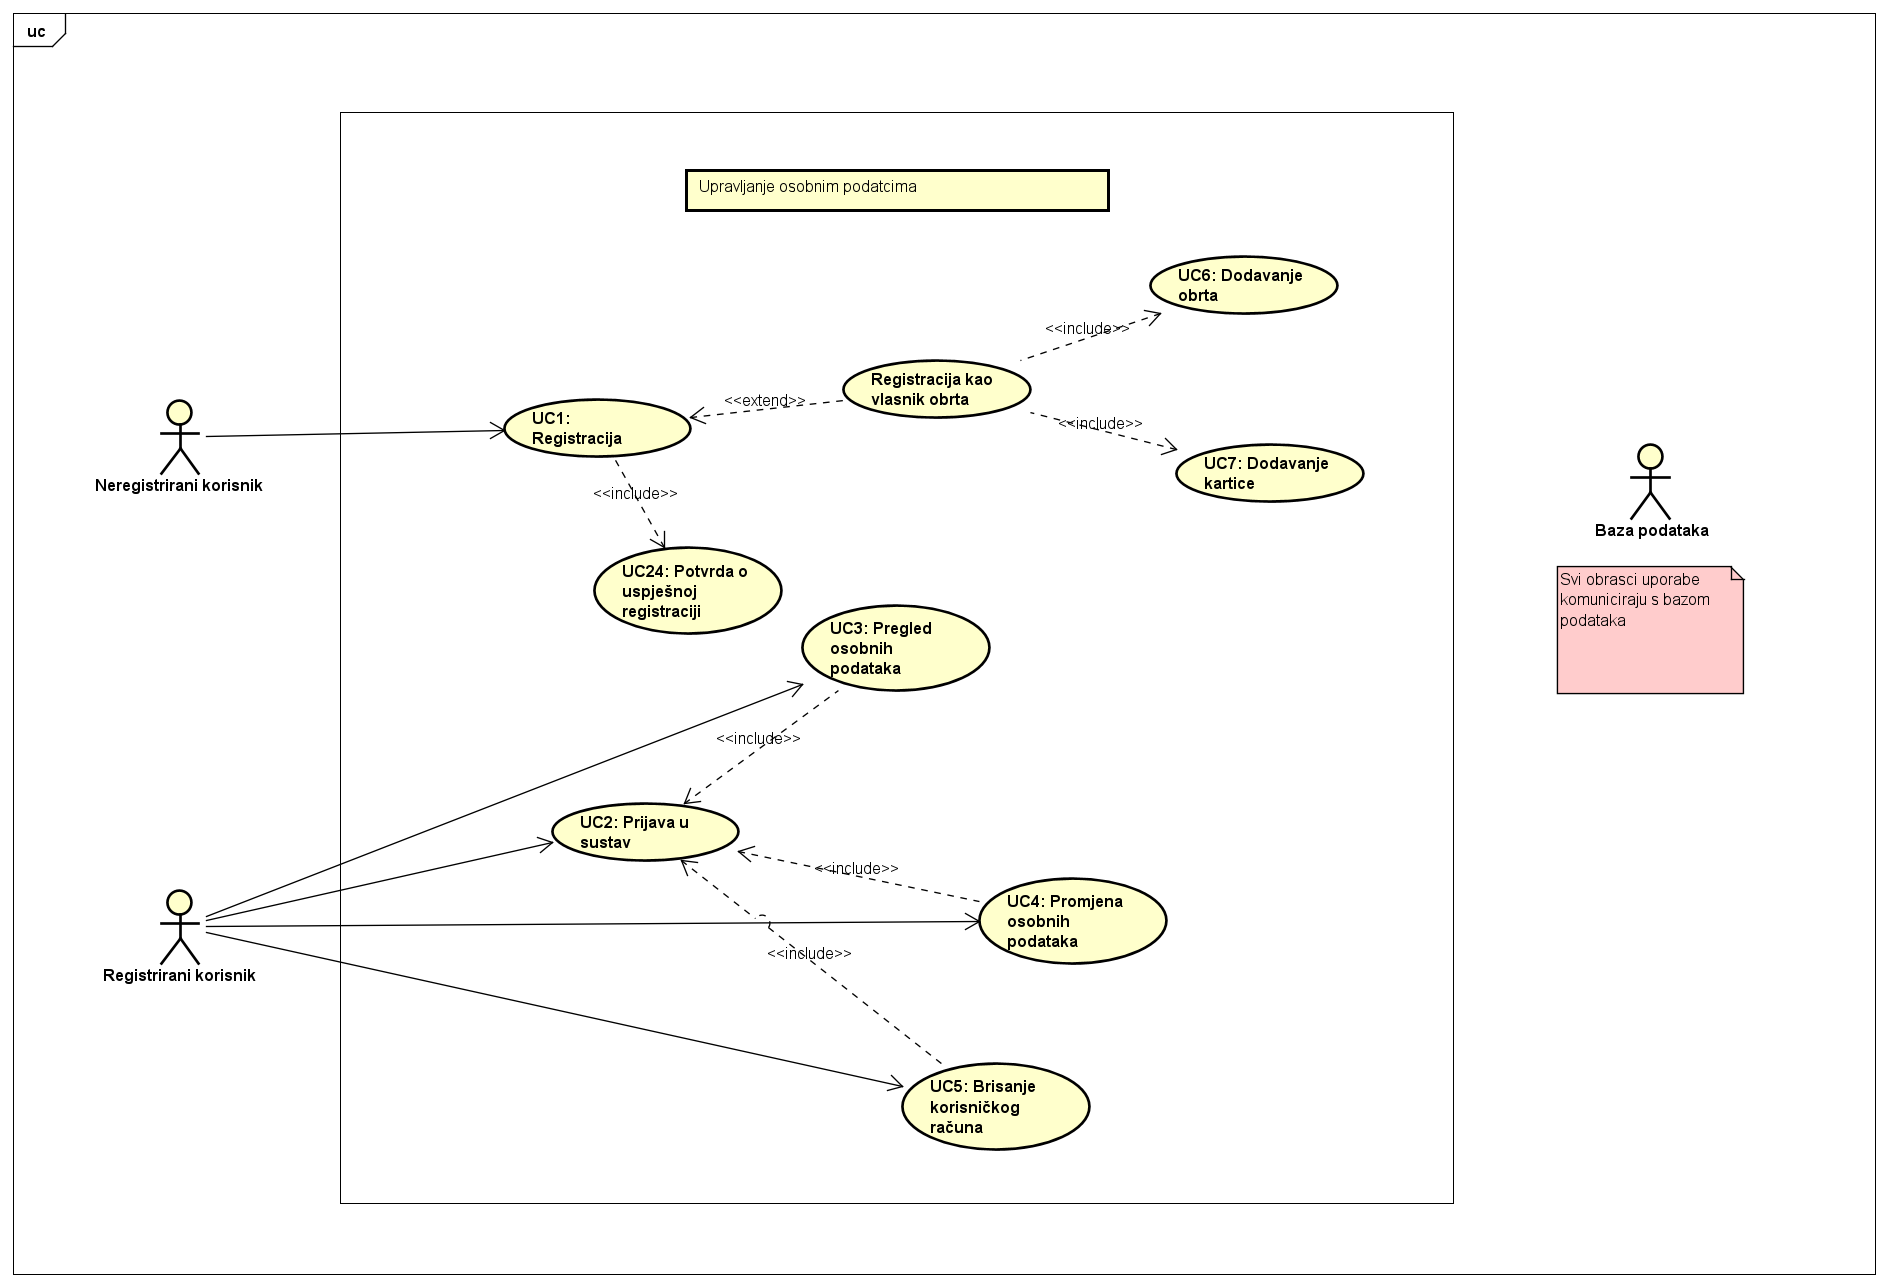
\includegraphics[width=\textwidth]{slike/dijagram1.png} 
			        \caption{Dijagram obrasca uporabe, upravljanje osobnim podatcima}
			    \label{fig:Upravljanje osobnim podatcima}
		    \end{figure}
		    
		    \begin{figure}[H]
			    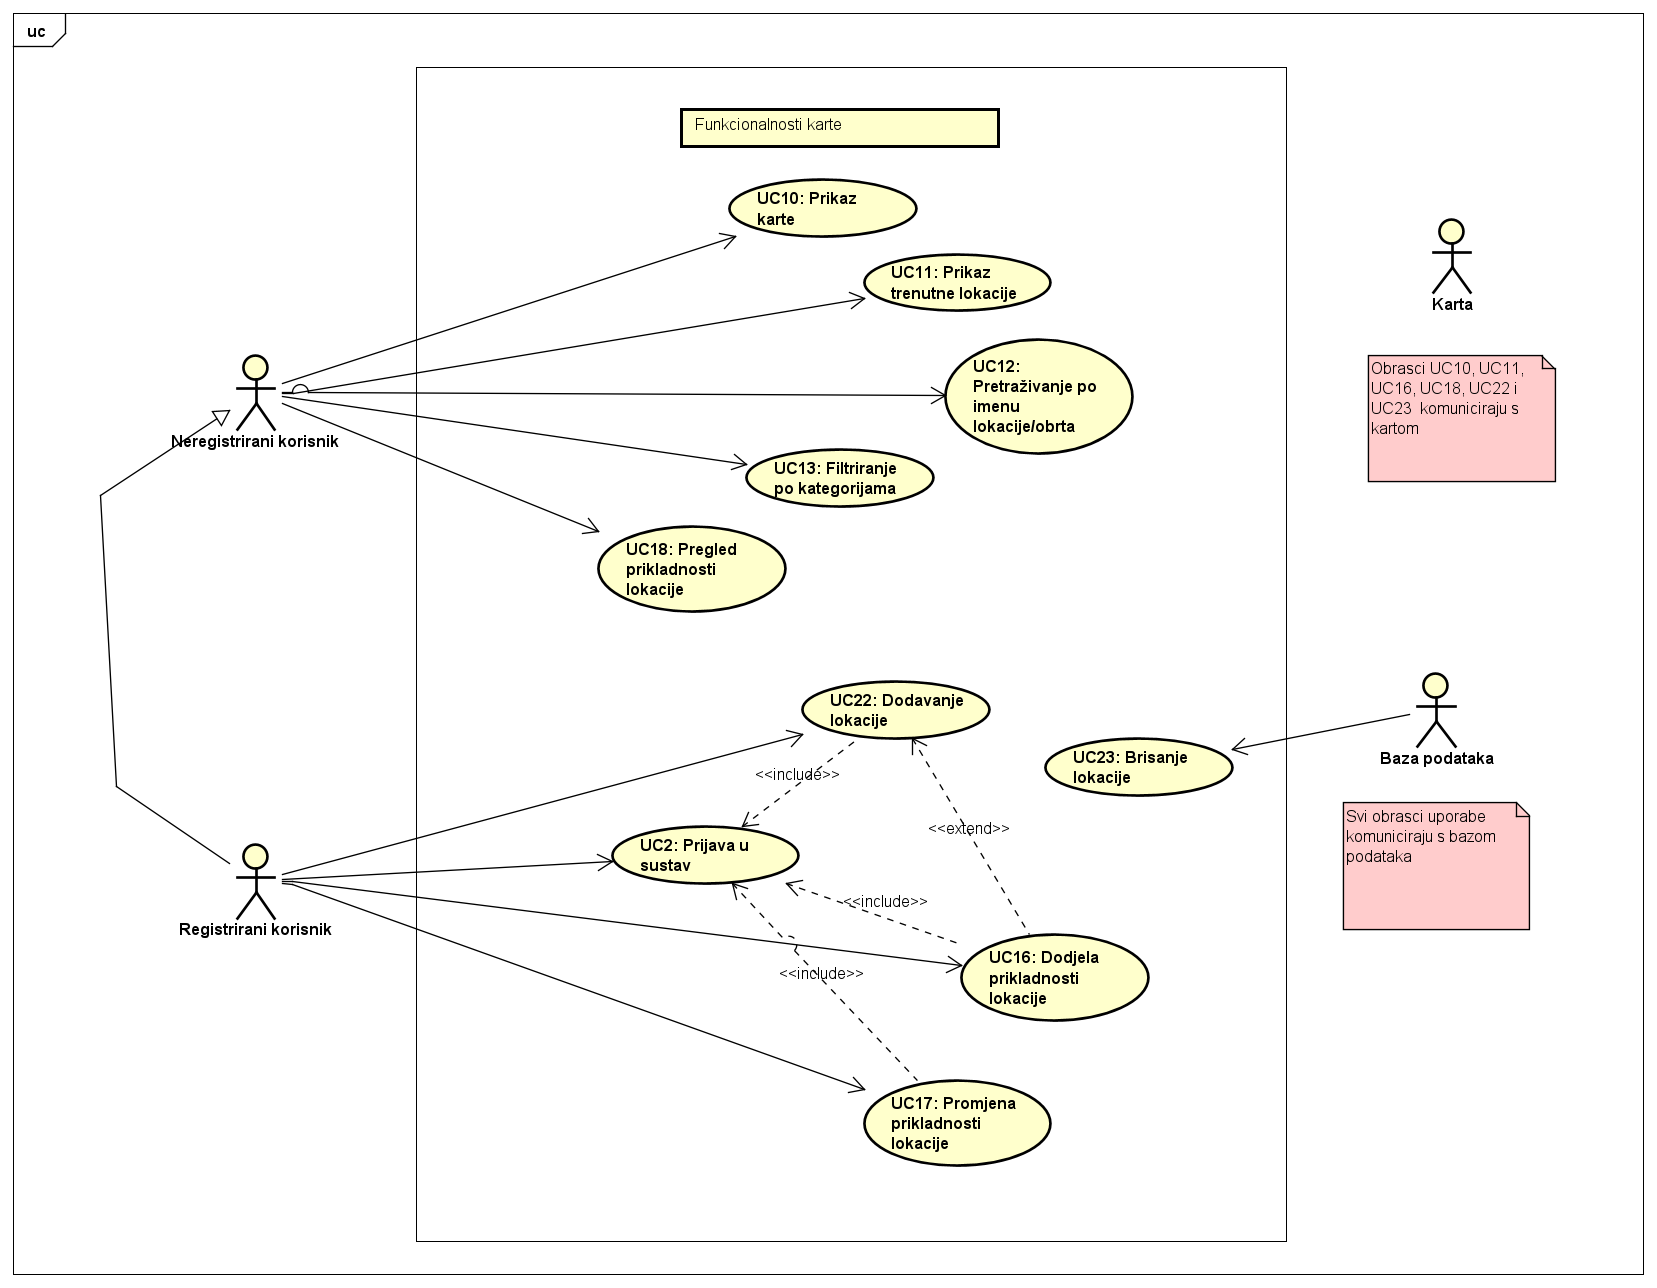
\includegraphics[width=\textwidth]{slike/dijagram2.png} 
			        \caption{Dijagram obrasca uporabe, funkcionalnost karte}
			    \label{fig:Funkcionalnosti karte}
		    \end{figure}
		    
		    \begin{figure}[H]
			    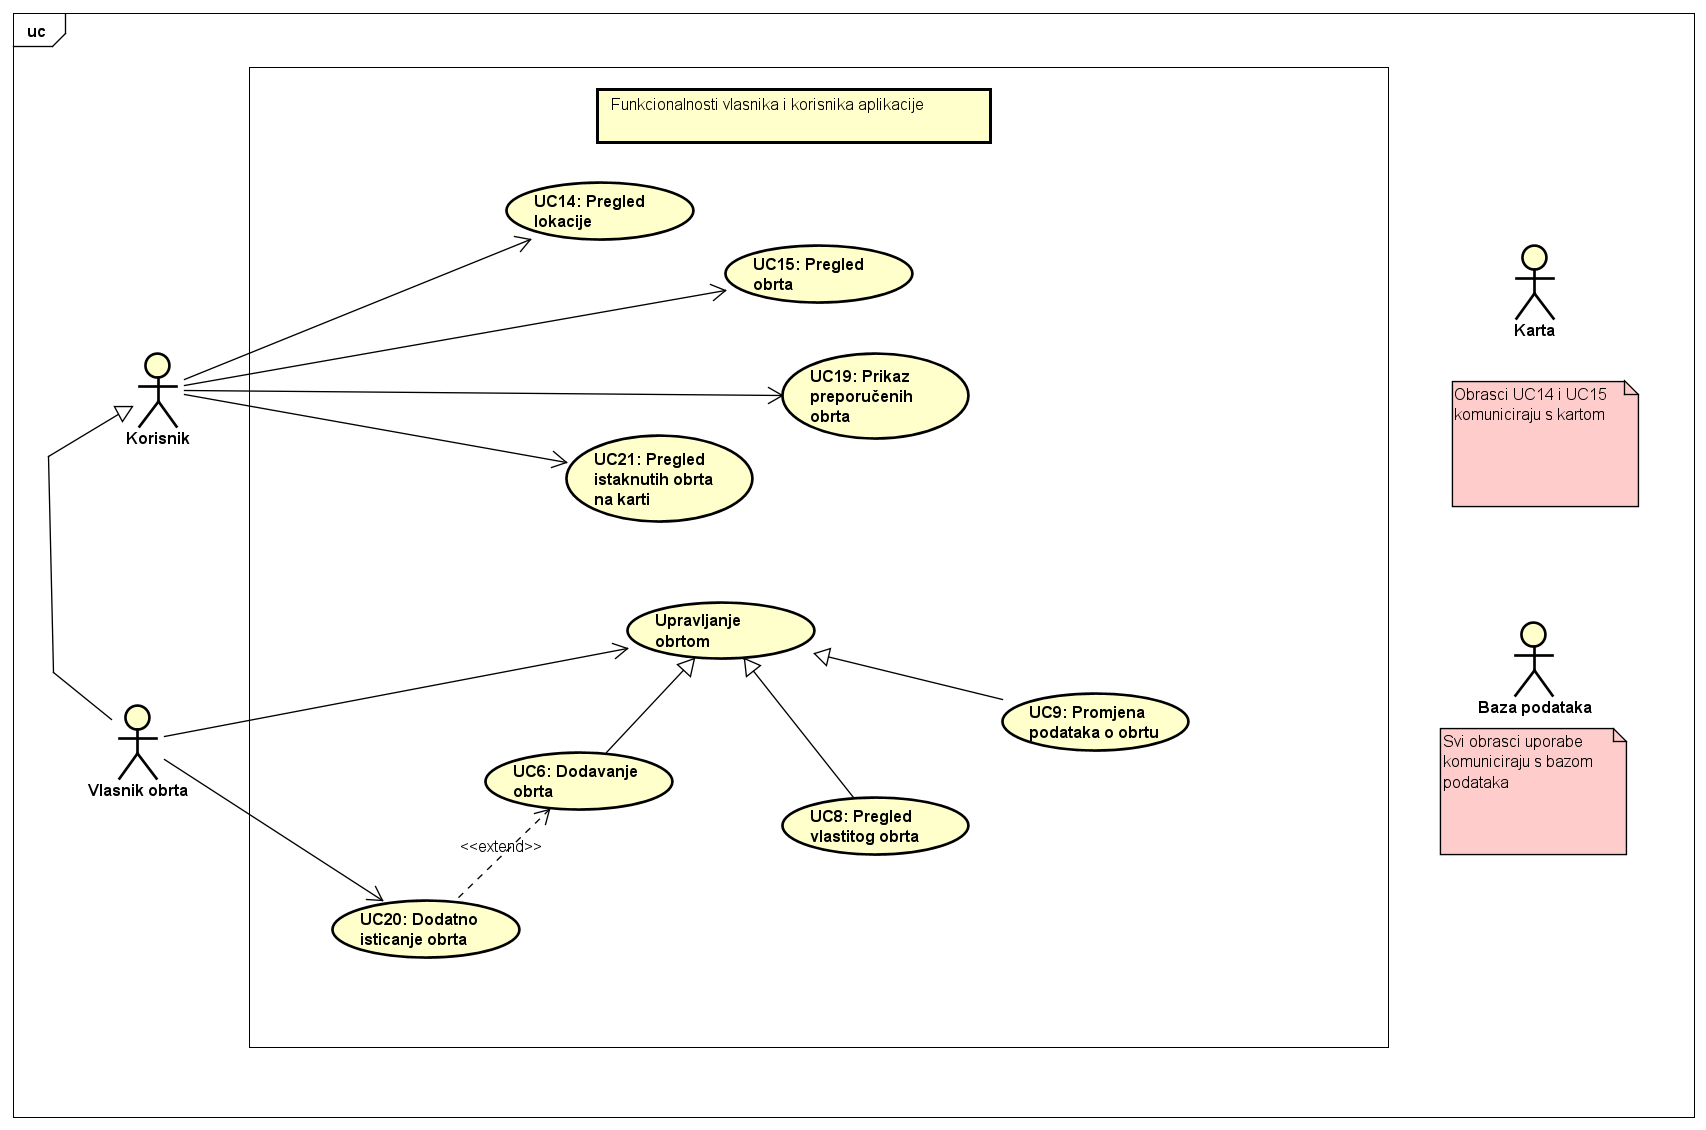
\includegraphics[width=\textwidth]{slike/dijagram3.png} 
			        \caption{Dijagram obrasca uporabe, funkcionalnost korisnika i vlasnika obrta}
			    \label{fig:Funkcionalnosti korisnika i vlasnika obrta}
		    \end{figure}

      \newpage
            
			\subsection{Sekvencijski dijagrami}
				
                \subsubsection{Obrazac uporabe UC5 – Brisanje korisničkog računa}
                 
                Registrirani korisnik odlazi na svoj profil gdje mu se prikazuju vlastiti podatci. Kako bi obrisao svoj profil korisnik mora poslati zahtjev za brisanjem računa i potvrditi da je siguran da ga želi obrisati. Ako je potvrdio brisanje onda se odmah brišu i sve njegove ocjene te ga aplikacija preusmjerava na početnu stranicu. Zatim se još u bazi podataka brišu sve lokacije koje više nemaju niti jednu ocjenu. 
               
                \begin{figure}[H]
			        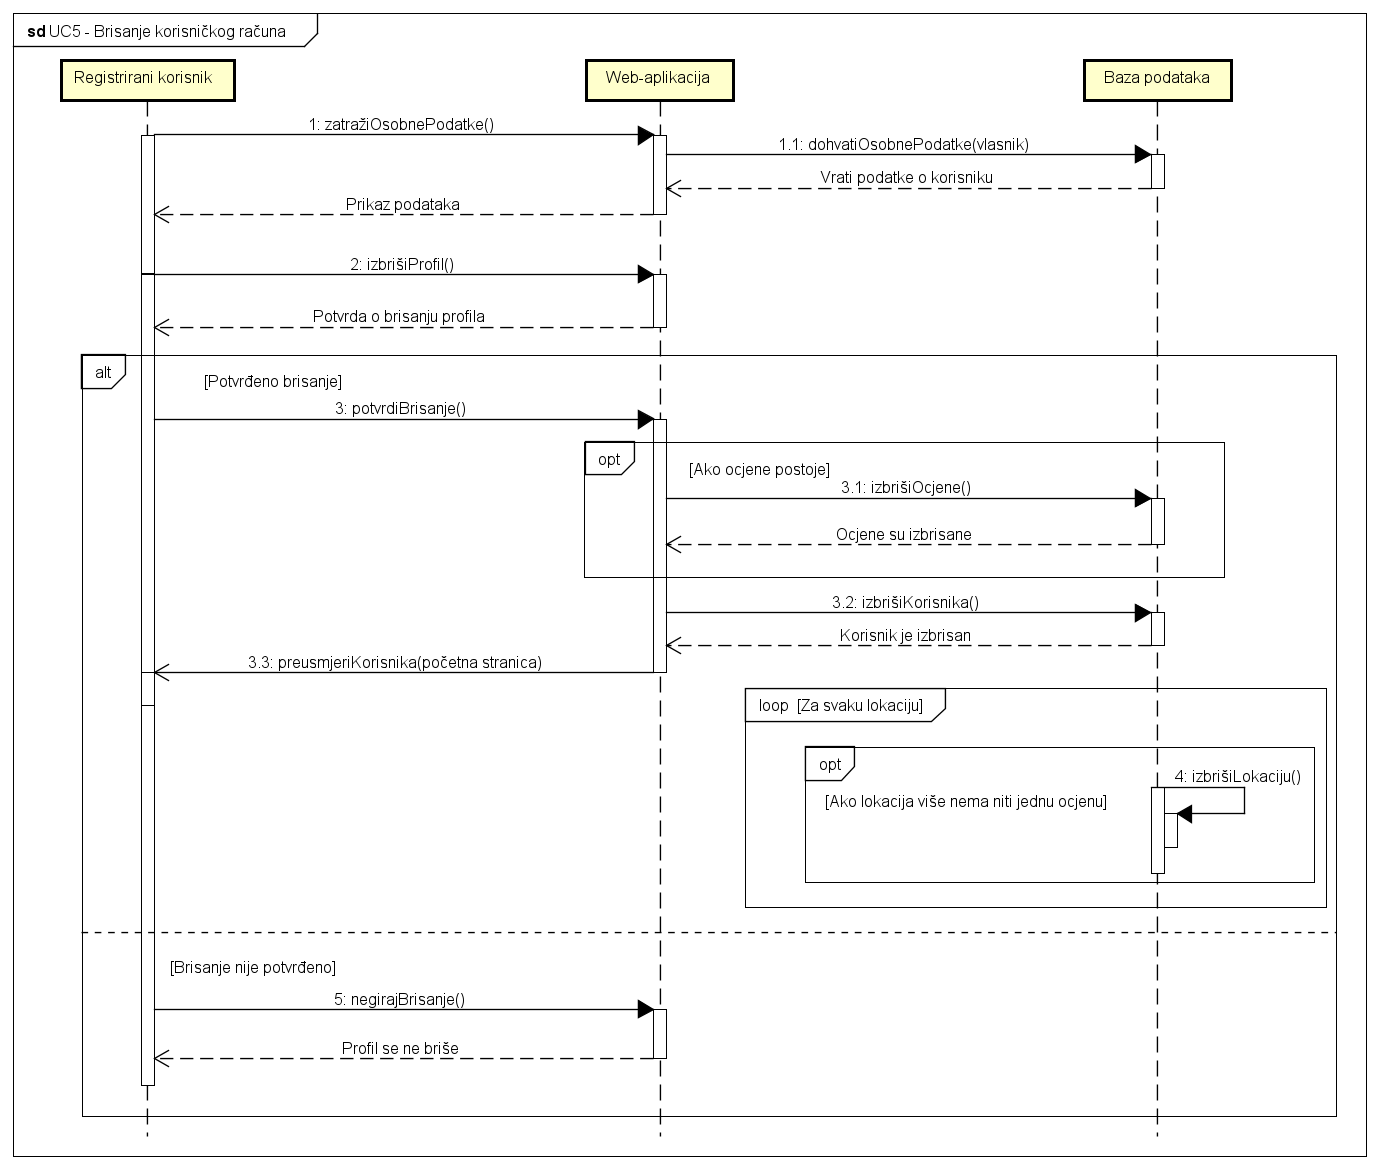
\includegraphics[width=\textwidth]{slike/sekvencijski1.png} 
			            \caption{Sekvencijski dijagram za UC5}
			        \label{fig:Sekvencijski dijagram za UC5}
		        \end{figure}

          \newpage
                
                \subsubsection{Obrazac uporabe UC12 – Pretraživanje lokacije/obrta po imenu}
	
	            Registrirani korisnik odlazi na kartu te mu baza podataka vraća sve lokacije, a karta ih onda prikazuje. Korisnik zatim upisauje lokaciju u tražilicu te mu baza podataka vraća rezultat pretrage. Ako je lokacije postojeća onda mu se karta centrira na traženu lokaciju. Uprotivnom karta se ne centrira.
	            
	            \begin{figure}[H]
			        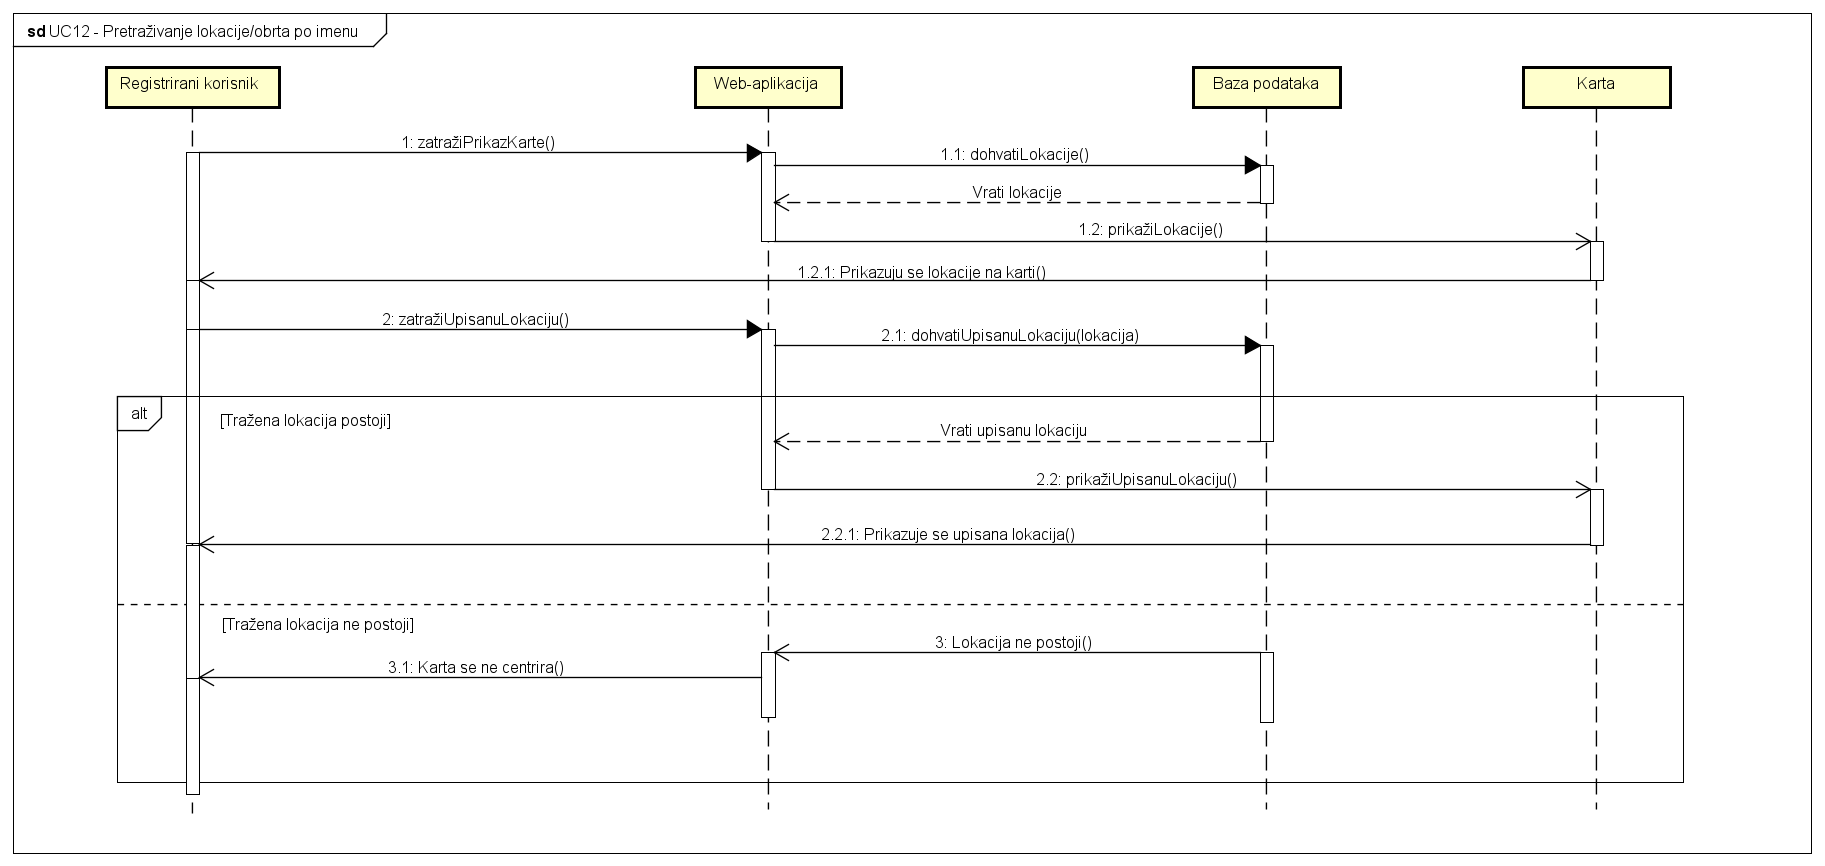
\includegraphics[width=\textwidth]{slike/sekvencijski2.png} 
			            \caption{Sekvencijski dijagram za UC12}
			        \label{fig:Sekvencijski dijagram za UC12}
		        \end{figure}

          \newpage
	            
	            \subsubsection{Obrazac uporabe UC20 – Promocija obrta}
	            Vlasnik obrta odlazi na svoj profil gdje mu se prikazuju vlastiti podatci. Odabire trajanje promocije te potvrđuje je li siguran da želi platiti za promociju obrta. Ako je potvrdio promociju trajanje promocije prikazuje mu se pod podatima o obrtu, u bazi podataka sprema se datum promocije i trajanje. U suprotnom mu se prikazuje da obrt nije promoviran.
	            
	            \begin{figure}[H]
			        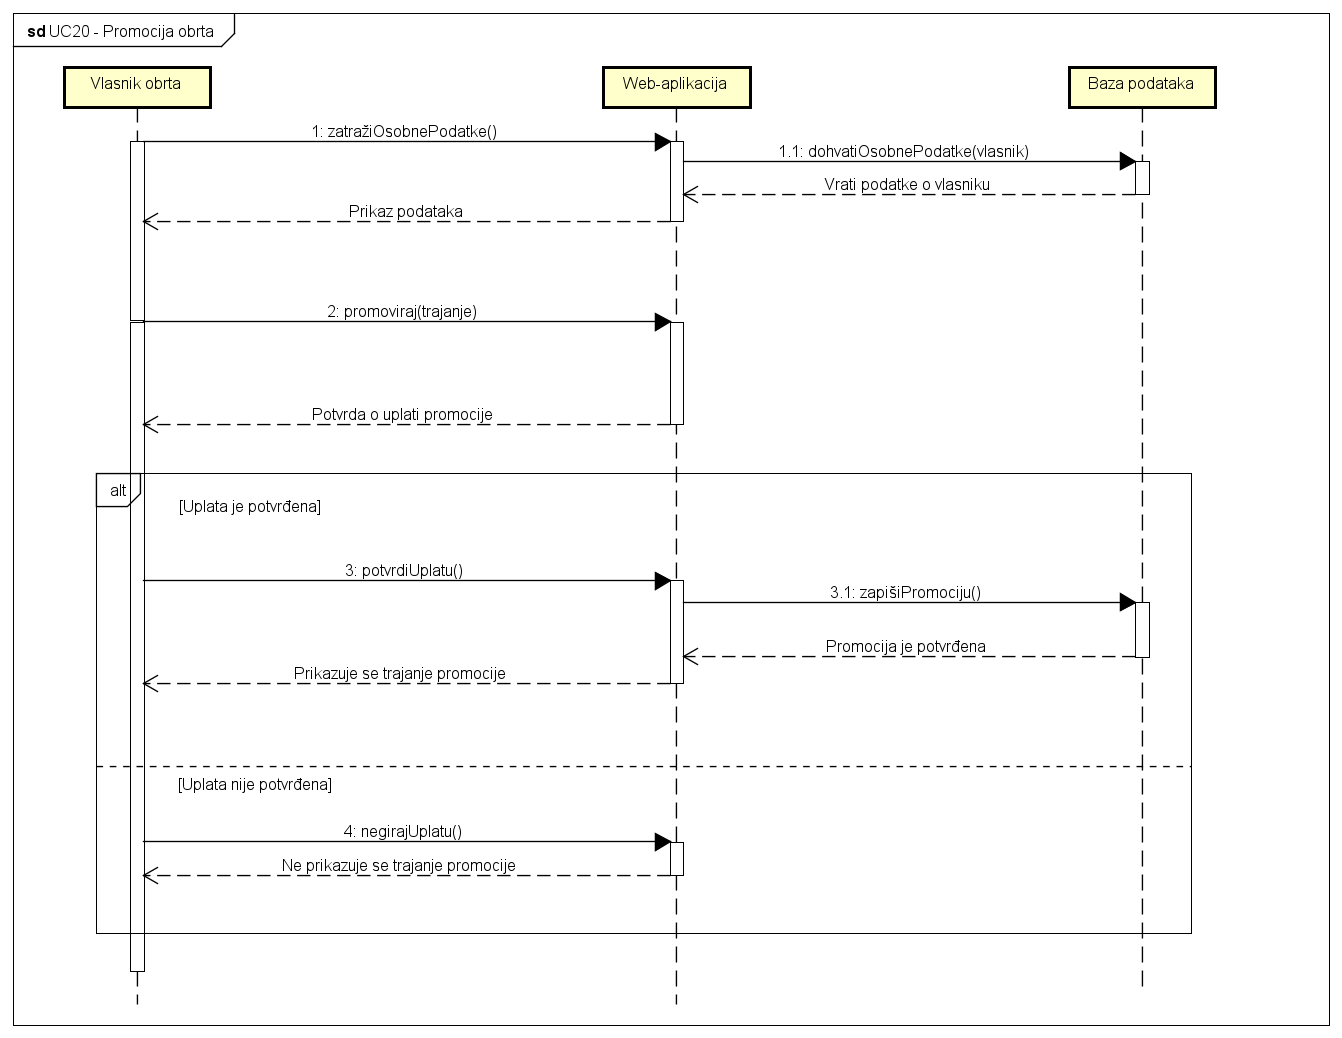
\includegraphics[width=\textwidth]{slike/sekvencijski3.png} 
			            \caption{Sekvencijski dijagram za UC20}
			        \label{fig:Sekvencijski dijagram za UC20}
		        \end{figure}

          \newpage
	            
		\section{Ostali zahtjevi}
		
		    \begin{itemize}
		        \item Aplikacija mora biti izvedena kao web aplikacija kojoj će korisnici pristupati uz pomoć korisničkog imena i lozinke
		        \item Oblikovanje aplikacije mora slijediti načela objektno-orijentiranog programiranja
		        \item Aplikacija mora biti prilagođena za različite veličine ekrana
		        \item Unos lokacija mora podržavati dijakritičke znakove hrvatske abecede
		        \item Aplikacija mora omogućiti rad više korisnika u stvarnom vremenu
		        \item Sustav kao valutu koristi euro
		        \item Aplikacija treba biti jednostavna za korištenje, a sučelje pregledno i intuitivno
		        \item Pristup bazi podataka ne bi trebao trajati duže od 5 sekundi
		    \end{itemize}
			 
	